\section{Simulation Study}
\label{sec:eval}

In this section, we use simulations to characterize the performance of each of our three recovery algorithms in terms of message and time overhead. 
Our goal is to illustrate the relative performance of our recovery algorithms over different topologies (e.g., \er graphs, Internet-like graphs) and across
different network conditions (e.g., topologies with fixed link costs, topologies with changing link costs, a single compromised node, and multiple compromised nodes).
%We count the number of messages required for nodes to find valid routing paths and count the number timesteps (epochs) for each algorithm to converge.

We build a custom simulator with a synchronous communication model: nodes send and receive messages at fixed epochs.  In each epoch, a node receives a
message from all its neighbors and performs its local computation.  In
the next epoch, the node sends a message (if needed).   All algorithms
are deterministic under this communication model.
The synchronous communication model, although simple, yields
interesting insights into the performance of each of the recovery algorithms. 
%Evaluation of our algorithms using a more general asynchronous communication model is left for future work, beyond the scope of this thesis.
%However, we believe an asynchronous implementation will demonstrate similar trends.  

We simulate the following scenario:
\begin{enumerate}
	\item Before $t'$, $\forall v \in V$ \minvv and \dmatrixv are correctly computed.

	\item At time $t'$, \bad is compromised and advertises a \badvector (a vector with a cost of $1$ to \emph{every} node in the network) to its neighboring nodes.

	\item The effect of \badvector spreads for a specified number of hops (this varies by experiment).  The variable $k$ refers to the number of hops that the effect of \badvector has spread.

	\item At time $t$, some node $v \in V$ notifies all $v \in adj($\bads$)$ that \bad was compromised. 
	{\footnote { \small For \cpr this node also indicates the time, $t'$, \bad was compromised.}} 

\end{enumerate}
The message and time overhead are measured in step (4) above. The pre-computation, described in Section \ref{subsec:preprocess}, is not counted towards message and time overhead
because all three recovery algorithms use this same procedure.

In order to keep this thesis proposal document brief, we only discuss a subset of our simulation results.  We focus on a simplified scenario in which a single compromised node
has distributed false routing state.  We consider \er graphs in cases where link costs remain fixed (Section \ref{subsec:simulation-fixed}) and link costs change (Section \ref{subsec:simulation-lc}).
The corresponding technical report \cite{TechRollback10}, discusses results using a richer simulation model that considers more realistic network conditions: an asynchronous communication model,
Internet-like graphs generated using GT-ITM \cite{GT-ITM} and Rocketfuel \cite{Rocketfuel}, and multiple compromised nodes.  We find that the trends discussed in this report hold when using these new topologies and 
additional simulation scenarios.
%Because we find the same trends hold in these additional scenarios, understanding this simplified scenario is instructive in 



\subsection{Simulations using Graphs with Fixed Link Weight}
\label{subsec:simulation-fixed}

Here we evaluate our recovery algorithms, in terms of message and time overhead, using \er graphs with fixed link weights. 
%We start with a simplified experiment setting to measure the message and time overhead incurred by each of the recovery algorithms. 
In particular, we consider Erd\"{o}s-R\'enyi graphs with parameters $n$ and $p$, where $n$ is the number of graph nodes and $p$ is the probability that link $(i,j)$ exists 
where $i,j \in V$. Link weights are selected uniformly at random between $[1,n]$.

In order to establish statistical significance, we generate several \er graphs to be used in our simulations. 
We iterate over different values of $k$. For each $k$, we  generate an Erd\"{o}s-R\'enyi graph, $G = (V,E)$, with parameters $n$ and $p$. Then we select a $v \in V$ uniformly at 
random and simulate the scenario described above, using $v$ as the compromised node. In total we sample $20$ unique nodes for each $G$.
We set $n=100$, $p=\{0.05,0.15,0.25, 0.25\}$, and let $k=\{1,2,... 10\}$. Each data point is an average over $600$ runs ($20$ runs over 
$30$ topologies).  

\begin{table}
\begin{center}
\begin{tabular}{|c|c|c|c|}
\hline
  $k=1$ & $k=2$ & $k=3$ & $k=4-10$ \\
\hline
  $554$ & $1303$ & $9239$ &  $12641$ \\
\hline
 %$p=0.05$  & $554$ & $1303$ & $9239$ &  $12641$ \\
\end{tabular}
\end{center}
\caption{Average number pairwise routing loops for \second in simulation described in Section \ref{subsec:simulation-fixed}.} 
%$p=.50$ for Experiment 1 is omitted because no pairwise routing loops are found across all $k$ values.} 
\label{tab:loop1}
\end{table}


Figure \ref{fig:msg-rand-p05} shows the message overhead as a function of $k$ when $p=.05$. The $90 \%$ confidence interval is included in the plot.
\cpr outperforms the other algorithms because \cpr removes false routing state with a single diffusing computation, rather than using an iterative process as in \second and \purges. 
\second performs poorly because of the \infinity problem: 
Table \ref{tab:loop1} shows the large average number of pairwise routing loops, an indicator of the occurrence of \infinity problem, \second encounters this simulation.
In addition, we counted the number of epochs in which at least one pairwise routing loop existed.  For \second (across all topologies), on average, all but the last three 
timesteps had at least one routing loop.  This suggests that the \infinity problem dominates the cost for \seconds. 
In contrast, no routing loops are found with \purge or \cprs, as expected.


However, \cprs's encouraging results should be interpreted with caution.
\cpr requires both loosely synchronized clocks and the time that node \bad was compromised to be identified, assumptions not required by \second nor \purges.  
Furthermore, this first simulation scenario is ideal for \cpr because fixed link costs ensure minimal stale state (i.e., residual \oldvector state)
after \cpr rolls back.  The next two simulations present more challenging and less favorable conditions for \cprs.





\begin{figure}[t]
\centering
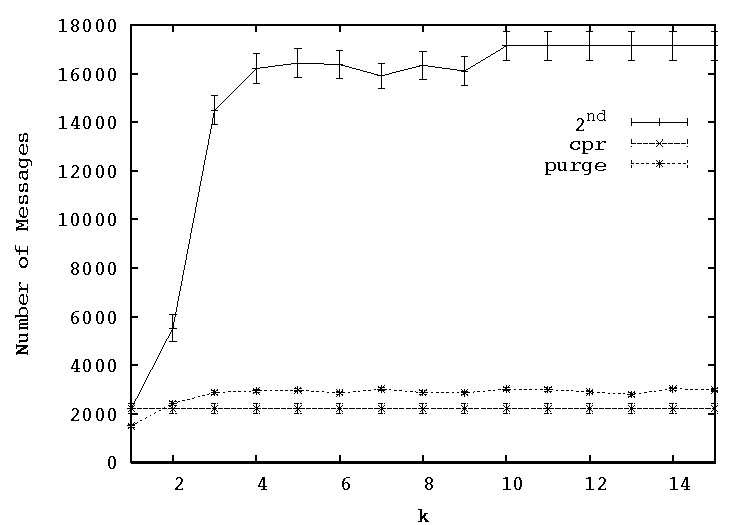
\includegraphics[width=0.49\textwidth]{figs/rollback-msg-rand5.pdf}
%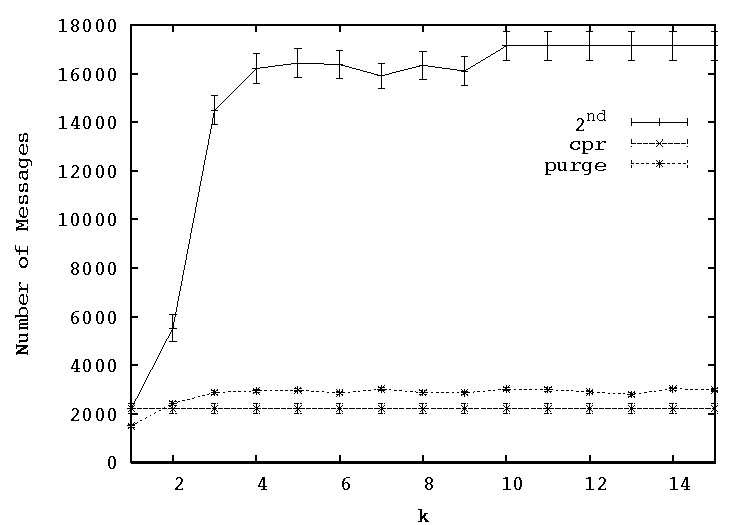
\includegraphics[scale=.35]{figs/rollback-msg-rand5.pdf}
\caption{Message overhead as function of the number of hops false routing state has spread from the compromised node ($k$), over \er graphs with fixed link weights.  The \er
graphs are generated using $n=100$, and $p=.05$, yielding an average diameter of $6.14$.}
\label{fig:msg-rand-p05}
\end{figure}



%\begin{figure*}[t]
%\centering

%\subfigure[{Message overhead for \er graph with link weights selected uniformly random from $[1,100]$. $p=.05$ and diameter=$6.14$.}]{ 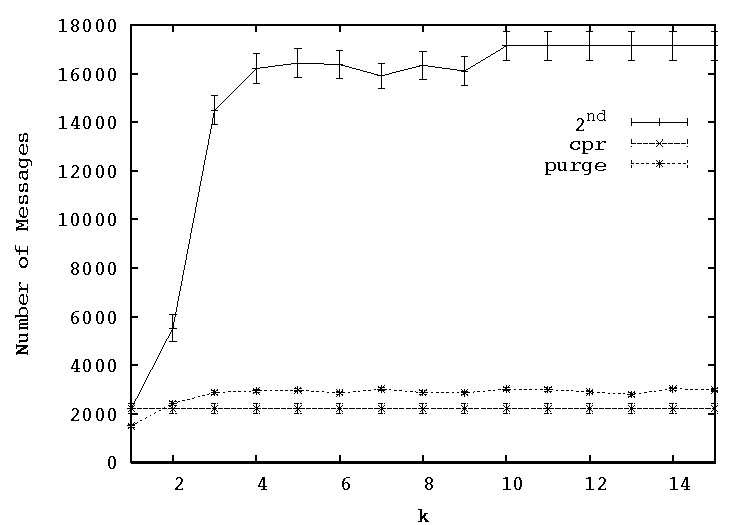
\includegraphics[scale=.35]{figs/rollback-msg-rand5.pdf}}
%\subfigure[{Message overhead for $p=0.05$ \er with link weights selected uniformly random with different $\lambda$ values. $z$ refers to the number of timesteps \cpr must rollback.}]
%	{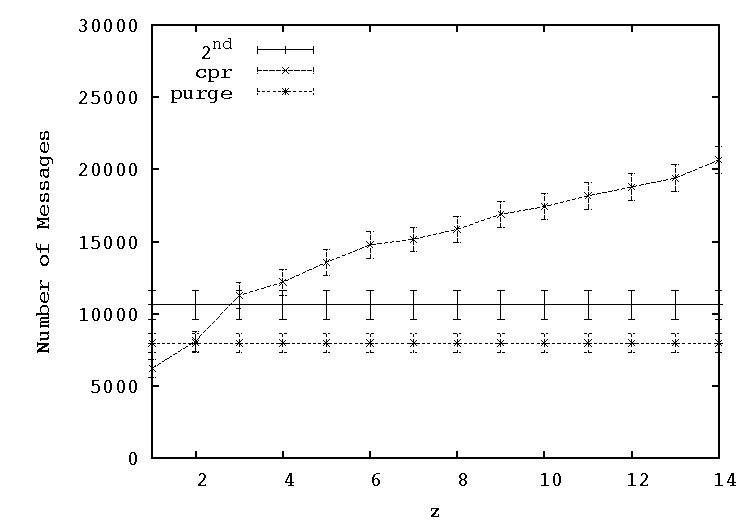
\includegraphics[scale=.35]{figs/rollback-p05-k4.pdf}} 

%\subfigure[{sim 1.}]{\label{fig:msg-rand-p05}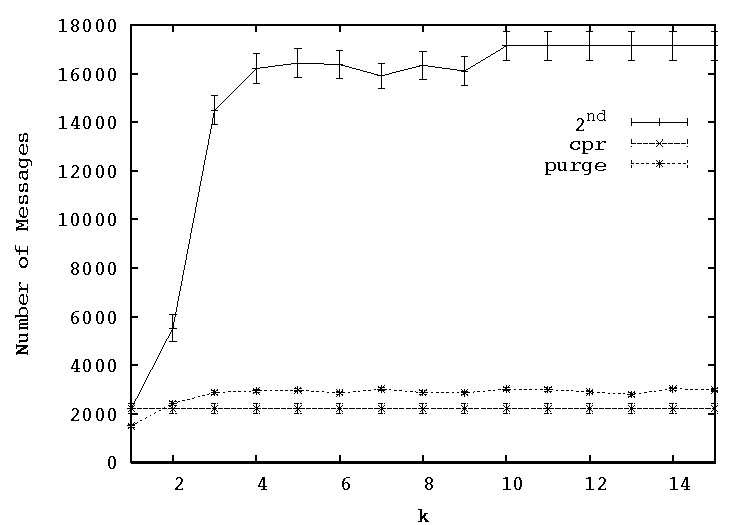
\includegraphics[scale=.55]{figs/rollback-msg-rand5.pdf}}
%\subfigure[{sim 2.}]{\label{fig:msg-checkpoint-p05}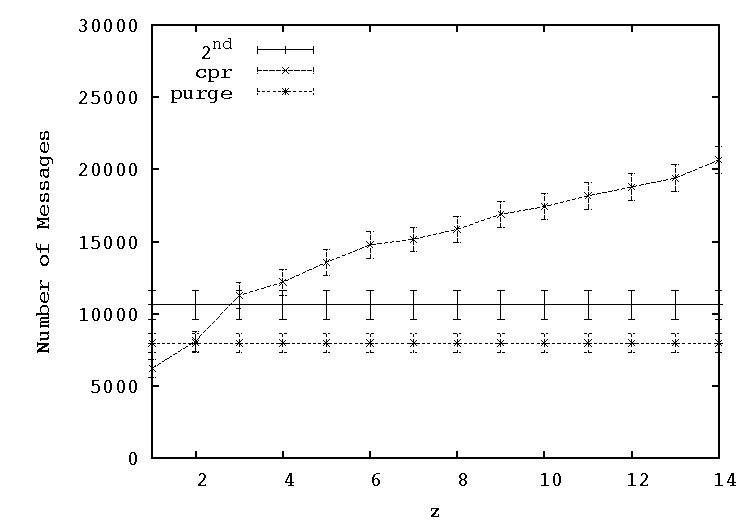
\includegraphics[scale=.55]{figs/rollback-p05-k4.pdf}} 
%\caption{Rollback simulations} 
%\label{fig:rollback-simulations}
%\end{figure*} 


%\begin{figure}[t]
%\centering
%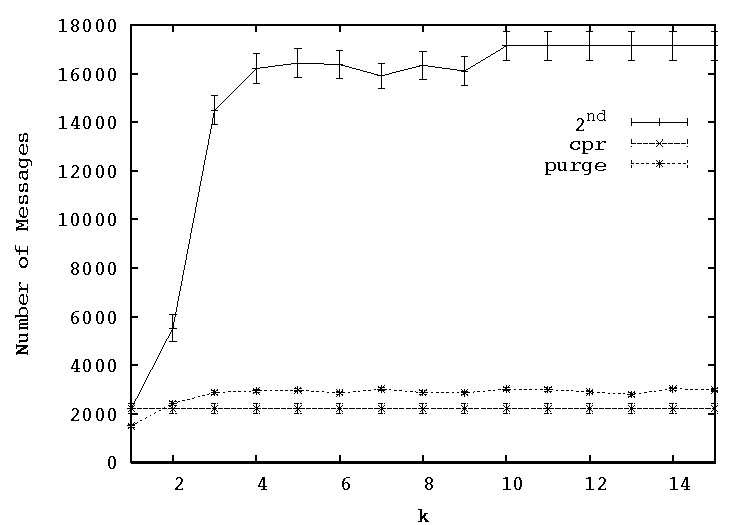
\includegraphics[scale=.35]{figs/rollback-msg-rand5.pdf}
%\caption{Message overhead for \er graph with link weights selected uniformly random from $[1,100]$. $p=.05$ and diameter=$6.14$.}
%\label{fig:msg-rand}
%\end{figure}







\subsection{Simulations using Graphs with Changing Link Weights}
\label{subsec:simulation-lc}

In the next two simulations we evaluate our algorithms over graphs with changing link costs. We introduce link cost changes between the time \bad is compromised and when \bad is discovered 
(e.g. during $[t',t]$). 
In particular, there are $\lambda$ link cost changes per timestep, where $\lambda$ is deterministic. 
To create a link cost change event, we modify links uniformly at random (except for all $(v,\bar{v})$ links), where the new link cost is selected uniformly at random from $[1,n]$. 


%\subsubsection{Experiment 4}

{\bf Effects of Link Cost Changes.}
Except for $\lambda$, our simulation setup is identical to that of the previous section. We let $\lambda = \{1,4,8\}$. In order to isolate the effects of link costs changes,
we assume that \cpr checkpoints at each timestep.

For the sake of brevity, we only show results for $n=100,p=.05, \lambda=4$ in Figure \ref{fig:lc-p05}.  
{\footnote {\small Our simulations for different $p$ values, yield the same trends.  Refer to our technical report for more details \cite{TechRollback10}.}}
\purge yields the lowest message overhead, but only slightly lower than \cprs. 
\cprs's message overhead increases with larger $k$ because there are more link cost change events to process. After \cpr rolls back, it must process all link cost
changes that occurred in $[t',t]$. 
In contrast, \second and \purge process some of the link cost change events during the interval $[t',t]$ as part of normal distance vector execution. 
%In our experimental setup, these messages are not counted because they do not occur in Step 4 (i.e., as part of the recovery process) of our simulation scenario described in Section \ref{sec:eval}.

Our analysis further indicates that \second performance suffers because of the \infinity problem. 
The gap between \second and the other algorithms shrinks as $\lambda$ increases because link cost changes have a larger effect on message overhead as $\lambda$ grows.



\begin{figure*}[t]
\centering
\subfigure[{Message overhead as a function of the number of hops false routing state has spread ($k$) 
where $\lambda=4$ link cost changes occur at each timestep.}]{\label{fig:lc-p05}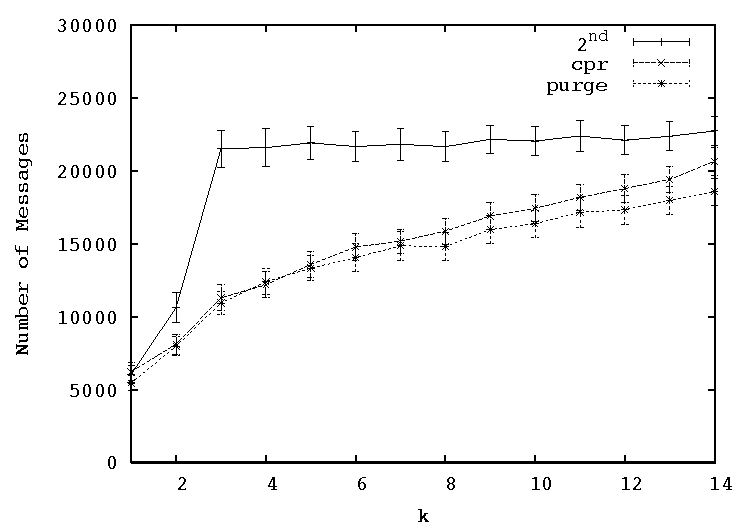
\includegraphics[width=0.49\textwidth]{figs/p05-lc4.pdf}}
\subfigure[{Message overhead as function of varying the checkpoint frequency, $z$. $z=0$ implies checkpointing occurs at every timestep, $z=1$ creates checkpoints every other timestamp, etc.}]
{\label{fig:msg-checkpoint-p05}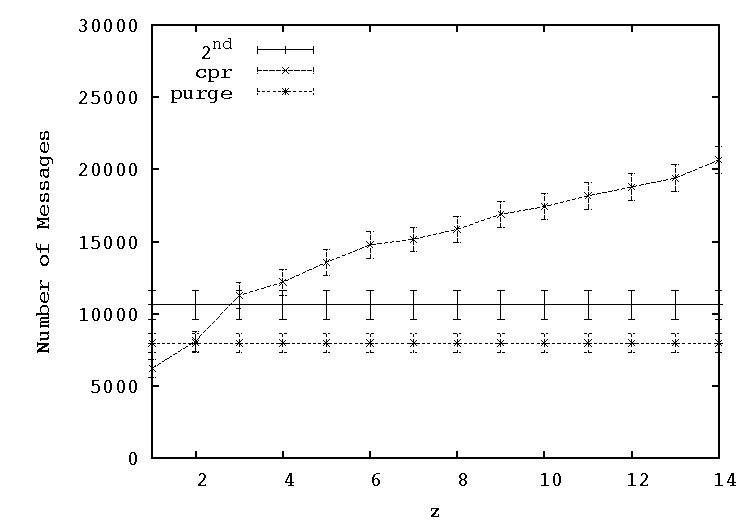
\includegraphics[width=0.49\textwidth]{figs/rollback-p05-k4.pdf}} 
%\subfigure[{sim 2.}]{\label{fig:msg-checkpoint-p05}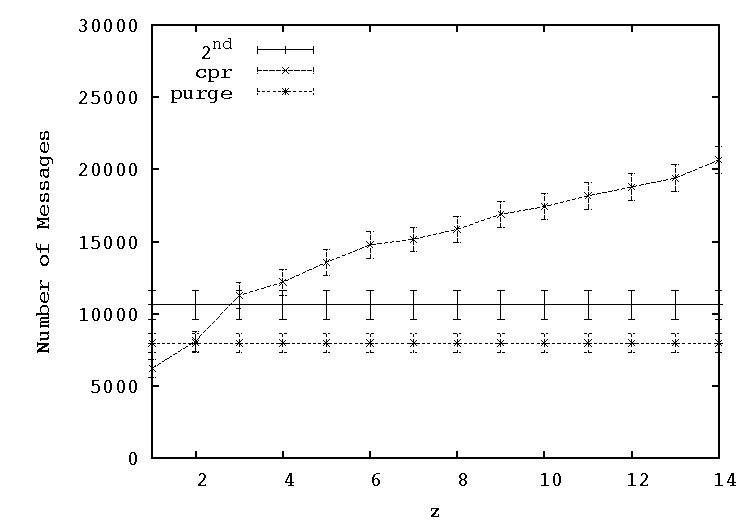
\includegraphics[scale=.55]{figs/rollback-p05-k4.pdf}} 
\caption{Section \ref{subsec:simulation-lc} plots.  Both plots consider \er graphs with changing link costs generated using $n=100$ and $p=.05$.
The average diameter of the generated graphs is $6.14$.}
%\caption{Message overhead for $p=0.05$ \er with link weights selected uniformly random with different $\lambda$ values.}
\label{fig:rollback-lc}
\end{figure*} 



%\subsubsection{Experiment 5}

{\bf Effects of Varying Checkpoint Frequency}.
In this simulation, we study the trade-off between message overhead and storage overhead for \cprs. To this end, we vary the frequency at which \cpr checkpoints and fix 
the interval $[t',t]$. Otherwise, our simulation setup is the same as the one just described (under the title ``Effects of Link Cost Changes''). %(\ref{subsec:simulation-lc}).

For conciseness, we only display a single plot.  Figure \ref{fig:msg-checkpoint-p05} shows the results for an \er graph with link weights selected
uniformly at random between $[1,n]$,
$n=100$, $p=.05$, $\lambda=4$ and $k=2$. We plot message overhead against the number of timesteps \cpr must rollback, $z$. \cprs's message overhead increases with larger $z$ 
because as $z$ increases there are more link cost change events to process. \second and \purge have constant message overhead because they operate independent of $z$.

We conclude that as the frequency of \cpr snapshots decreases, \cpr incurs higher message overhead.  Therefore, when choosing the frequency of checkpoints,
the trade-off between storage and message overhead must be carefully considered. 


%\begin{figure}[t]
%\centering
%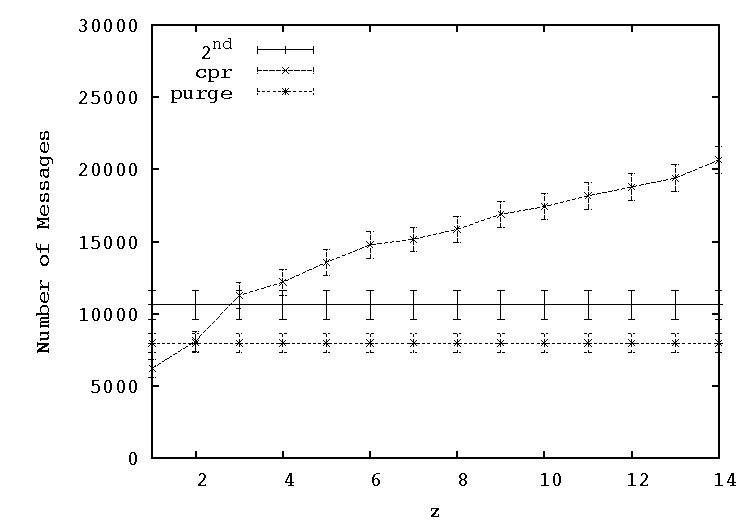
\includegraphics[scale=.35]{figs/rollback-p05-k4.pdf}
%\caption{Message overhead for $p=0.05$ \er with link weights selected uniformly random with different $\lambda$ values. $z$ refers to the number of timesteps \cpr must rollback.}
%\label{fig:lc-fixk}
%\end{figure} 






\subsection{Summary of Simulation Results}
\label{subsec:discuss}

Our results show that for graphs with fixed link costs, \cpr yields the lowest message and time overhead. \cpr benefits from removing false state with a single
diffusing computation. However, \cpr has storage overhead, requires loosely synchronized clocks, and requires the time that node \bad was compromised to be identified.

\seconds's performance is determined by the \infinity problem. \purge avoids the \infinity problem by first globally invalidating false state.  Therefore in cases where the \infinity problem is 
significant, \purge outperforms \seconds.

When considering graphs with changing link costs, \cprs's performance suffers because it must process all valid link cost changes that occurred since \bad was compromised.
Meanwhile, \second and \purge make use of computations that followed the injection of false state, that do not depend on false routing state. However, \seconds's performance degrades 
because of the \infinity problem.  \purge eliminates the \infinity problem and therefore yields the best performance over topologies with changing link costs.

Finally, we found that an additional challenge with \cpr is setting the parameter that determines the checkpoint frequency.
More frequent checkpointing yields lower message and time overhead at the cost of more storage overhead. Ultimately, application-specific factors must be considered
when setting this parameter. 

